En VirtualBox, aunque se instalamos más de una aplicación como fake gps (figura 17):


        \begin{figure}[H]
  \begin{center}
    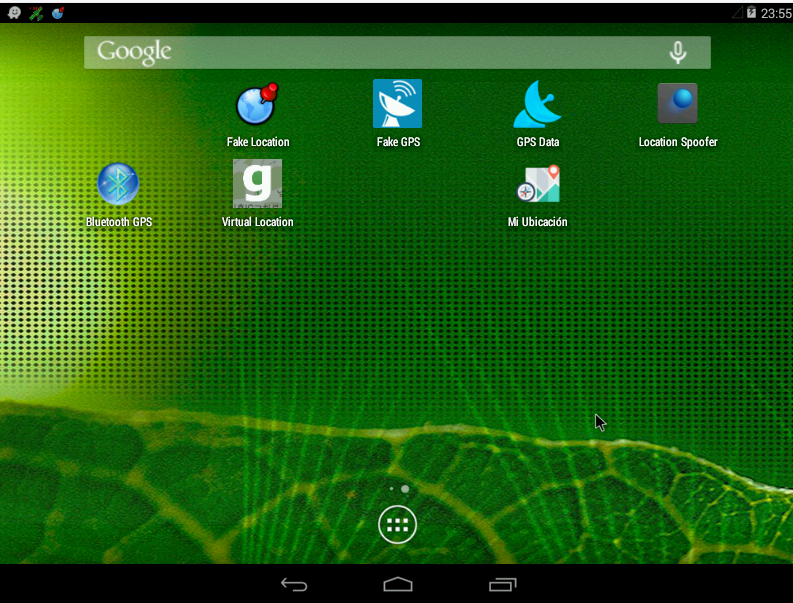
\includegraphics[width=0.6\textwidth]{imagenes/fig31.png}
    \caption{Aplicaciones instaladas para fakegps}
  \end{center}
\end{figure}


Waze no mostró el mapa, como se ve en la figura 20:

        \begin{figure}[H]
  \begin{center}
    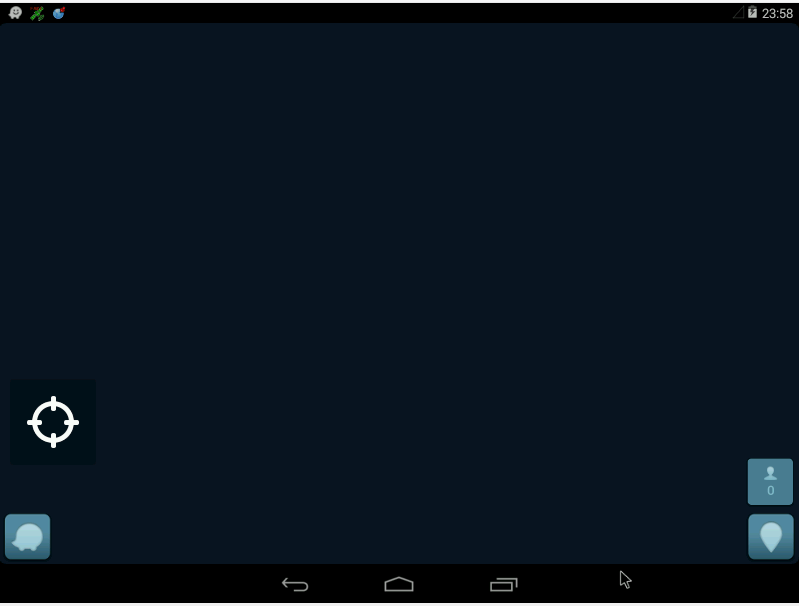
\includegraphics[width=0.6\textwidth]{imagenes/fig32.png}
    \caption{Waze no muestra mapa en maquina virtual (VirtualBox) }
  \end{center}
\end{figure}

En la máquina virtual al enviar una alerta, no aparece el mensaje de alerta enviada, figura 19:

        \begin{figure}[H]
  \begin{center}
    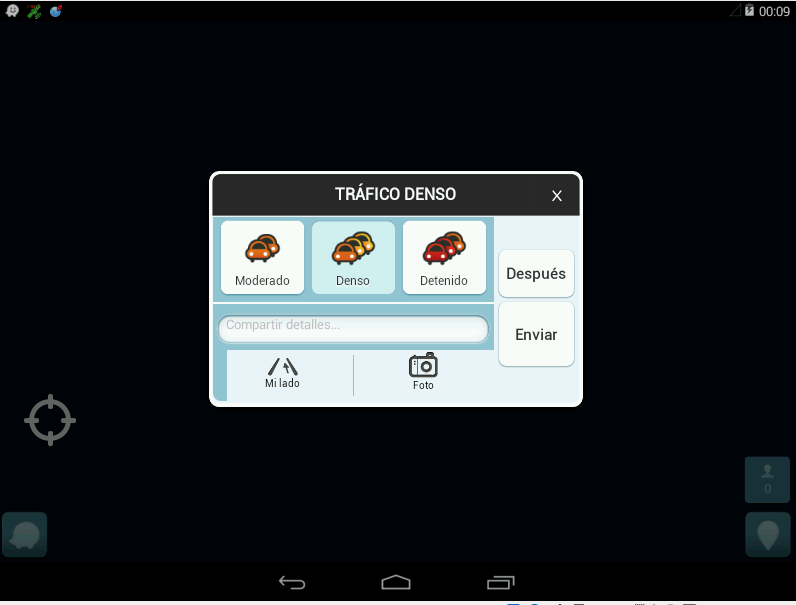
\includegraphics[width=0.6\textwidth]{imagenes/fig33.png}
    \caption{En la maquina virtual no se muestra el mensaje de alerta enviada}
  \end{center}
\end{figure}

Como es el caso de enviar una alerta desde un celular:

        \begin{figure}[H]
  \begin{center}
    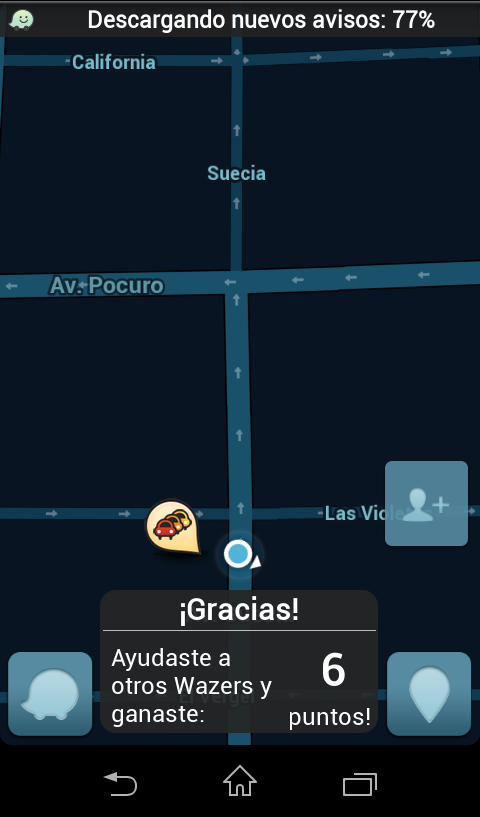
\includegraphics[width=0.3\textwidth]{imagenes/fig34.png}
    \caption{Mensaje de alerta enviada mostrada en un celular}
  \end{center}
\end{figure}

Otra opción descartando VirtualBox, fue probar con el emulador de android BlueStacks:

        \begin{figure}[H]
  \begin{center}
    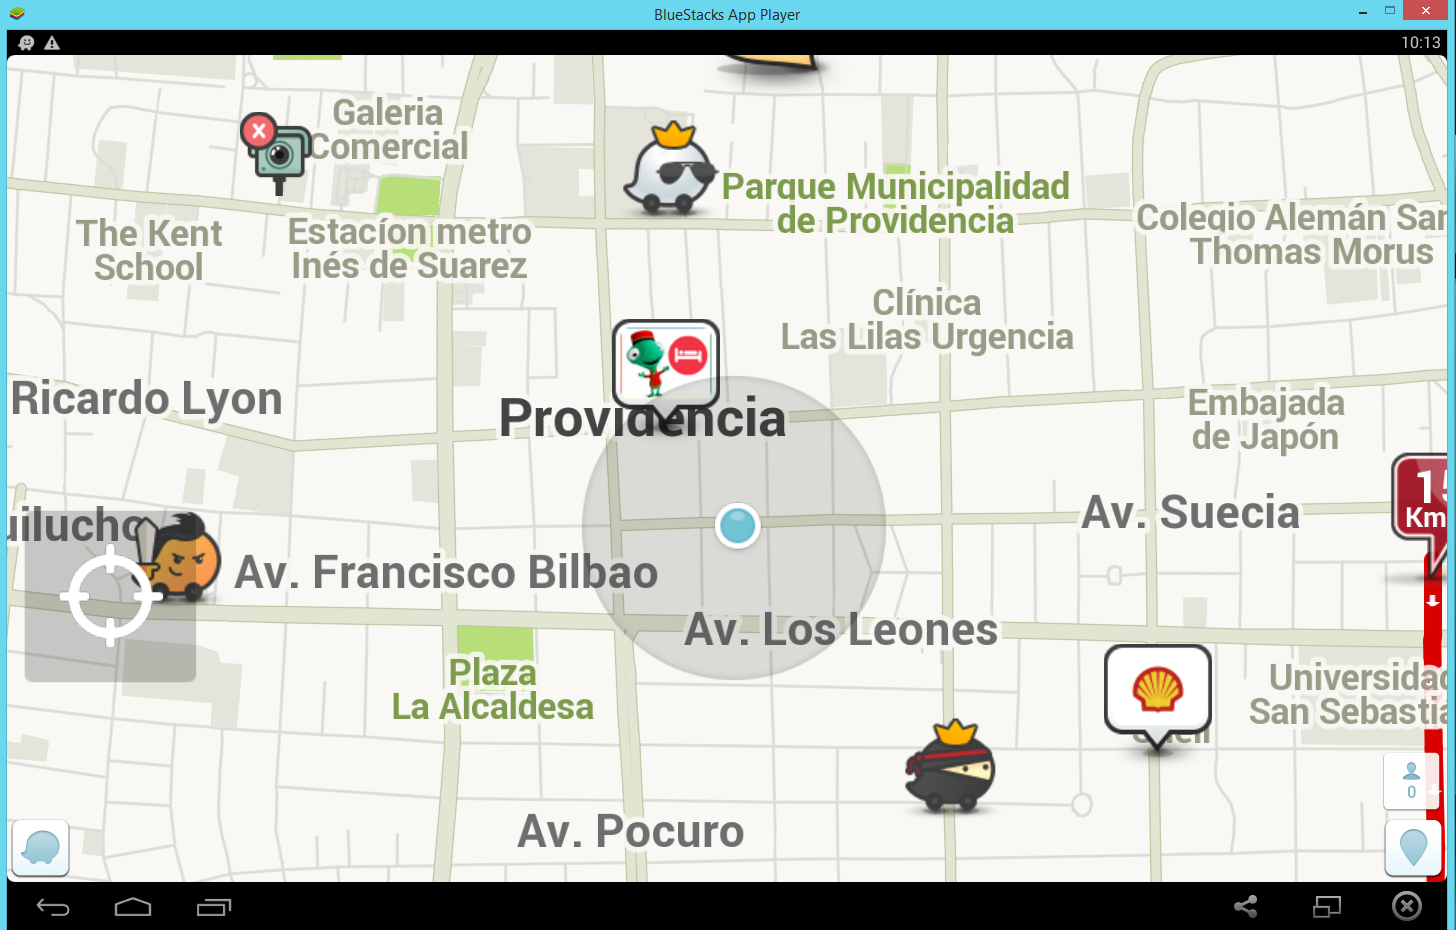
\includegraphics[width=0.7\textwidth]{imagenes/fig35.png}
    \caption{Waze en el emulador de Android Bluestacks}
  \end{center}
\end{figure}

En este caso si se muestra el mapa, y también es posible enviar una alerta:

        \begin{figure}[H]
  \begin{center}
    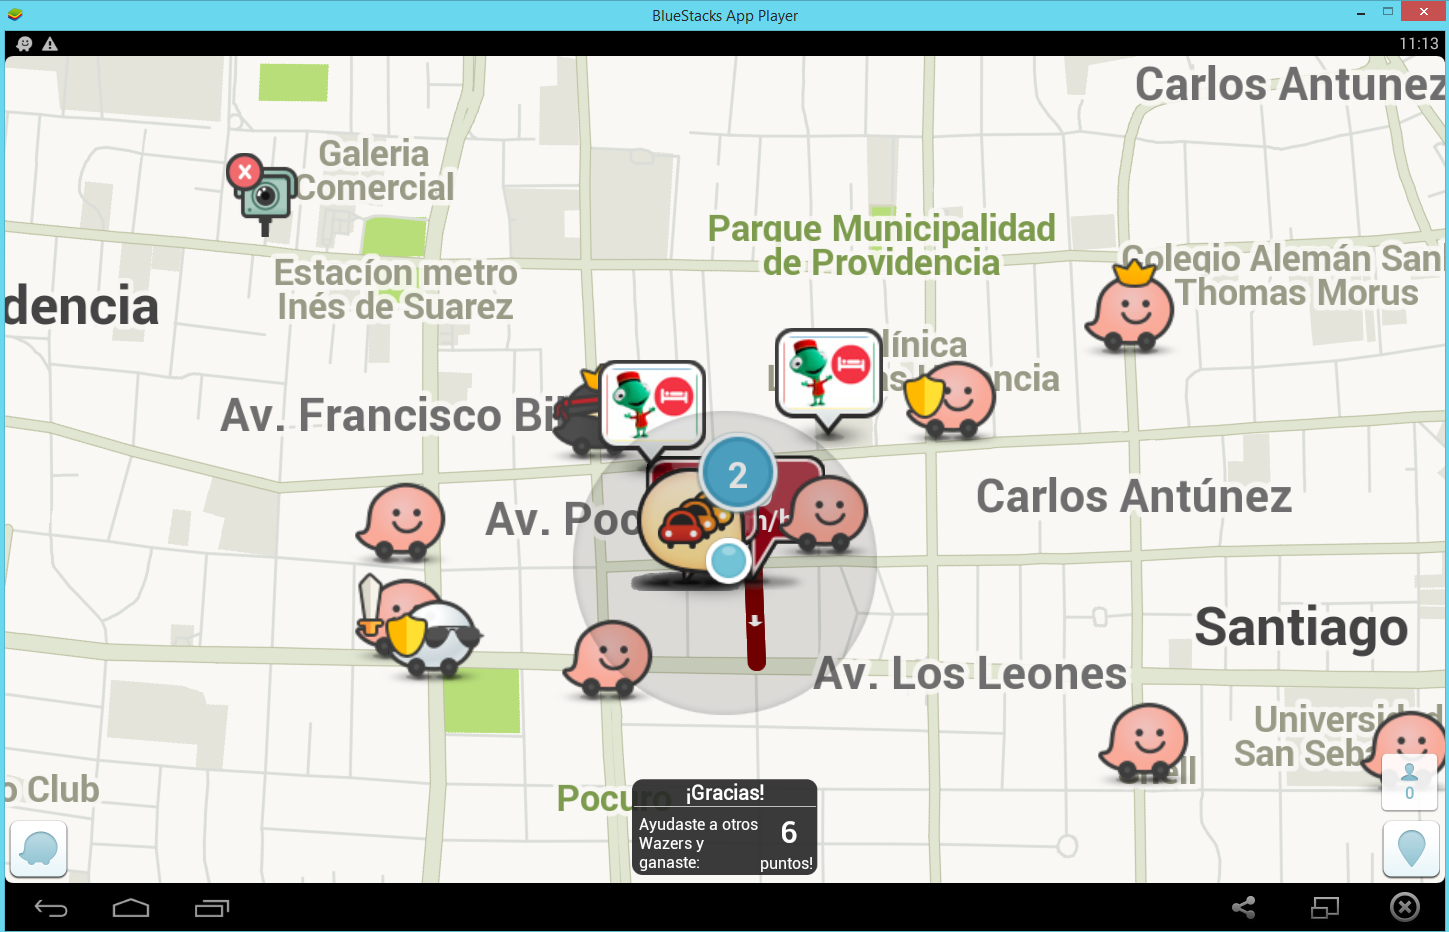
\includegraphics[width=0.7\textwidth]{imagenes/fig36.png}
    \caption{En Bluestack, Waze si muestra el mapa como en un celular}
  \end{center}
\end{figure}


y luego de enviarla aparece en el celular:

        \begin{figure}[H]
  \begin{center}
    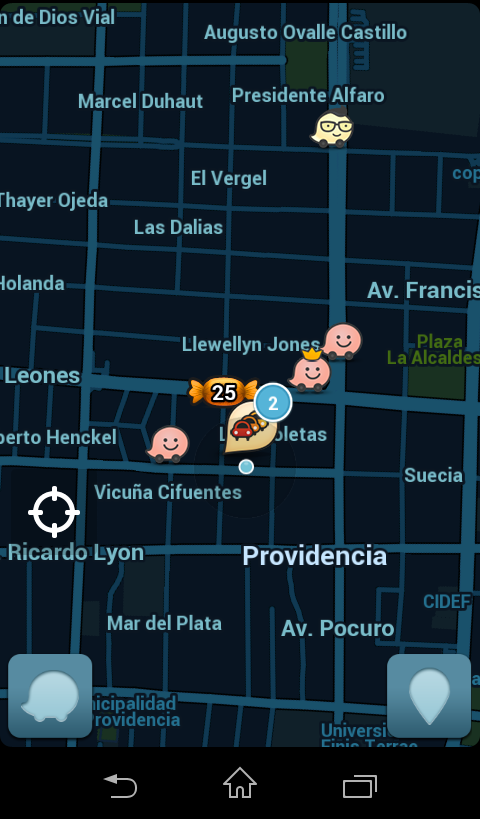
\includegraphics[width=0.3\textwidth]{imagenes/fig37.png}
    \caption{Alerta enviada usando Bluestacks aparece se muestra en un celular}
  \end{center}
\end{figure}

El problema que encontramos con BlueStacks fue que no es posible acceder a los archivos de la aplicación desde afuera. Pero si en la máquina virtual de Android:

        \begin{figure}[H]
  \begin{center}
    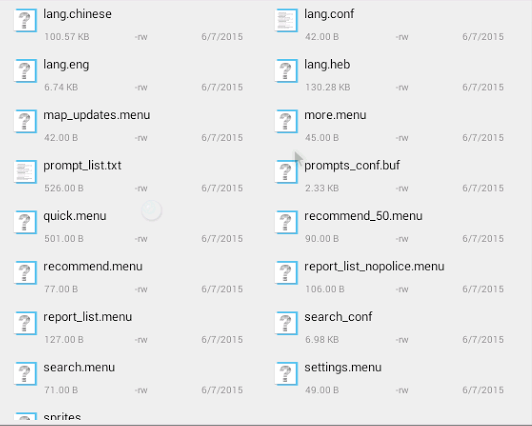
\includegraphics[width=0.7\textwidth]{imagenes/fig38.png}
    \caption{Archivos de Waze dentro de la maquina virtual}
  \end{center}
\end{figure}

        \begin{figure}[H]
  \begin{center}
    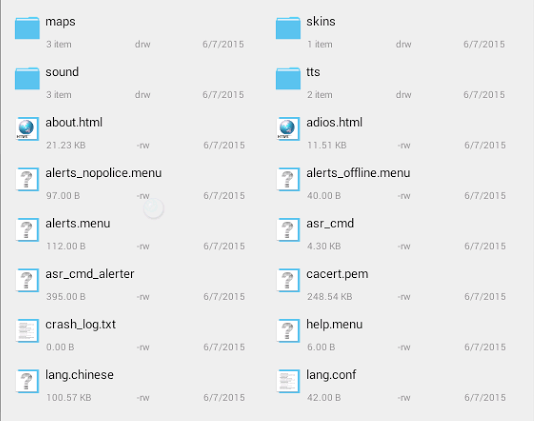
\includegraphics[width=0.7\textwidth]{imagenes/fig39.png}
    \caption{Más archivos de Waze dentro de la máquina virtual}
  \end{center}
\end{figure}

Dentro de los archivos no se encontró nada configurable. El archivo lang.conf solo mantenía los nombres de los lenguajes disponibles del software. [Figura 26 y 27]

En los archivos menús al parecer mantiene llamadas a funciones de Waze, ya que solo mantiene líneas con nombres de acciones aparentemente. [Figura 26]

        \begin{figure}[H]
  \begin{center}
    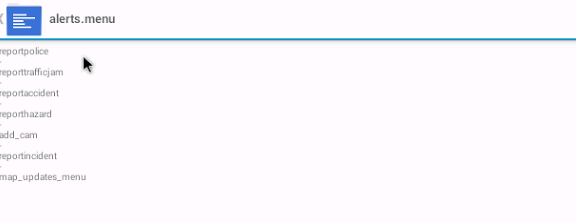
\includegraphics[width=0.9\textwidth]{imagenes/fig40.png}
    \caption{Contenido archivo alerts.menu}
  \end{center}
\end{figure}

De todas formas, intentamos modificar para ver si esto tiene incidencias en la aplicación, modificando el mismo archivo de alertas con uno similar:


        \begin{figure}[H]
  \begin{center}
    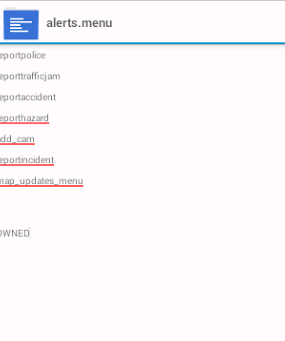
\includegraphics[width=0.6\textwidth]{imagenes/fig41.png}
    \caption{Archivo alerts.menu modificado}
  \end{center}
\end{figure}

Pero esto no tuvo repercusiones en la aplicación:


        \begin{figure}[H]
  \begin{center}
    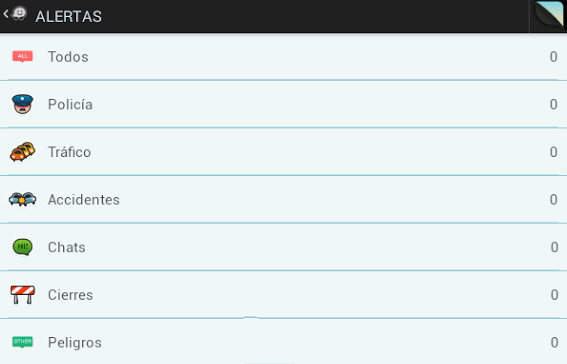
\includegraphics[width=0.6\textwidth]{imagenes/fig42.png}
    \caption{Menu de alertas no es afectado por la modificación del archivo alerts.menu}
  \end{center}
\end{figure}


Se volvió a verificar la aplicación y esta había reemplazado el archivo alerts.menu con el archivo original, por tanto, podemos deducir que la aplicación genera estos ficheros al iniciar.
\\\\
Se volvió a verificar la aplicación y esta había reemplazado el archivo alerts.menu con el archivo original, por tanto, podemos deducir que la aplicación genera estos ficheros al iniciar.
\\\\
Para verificar si la aplicación se ve alterada al modificar estos mismos archivos mientras corre, se instaló SSHelper[21] para poder entrar mediante SSH al dispositivo y modificar los archivos mientras corría la aplicación.


        \begin{figure}[H]
  \begin{center}
    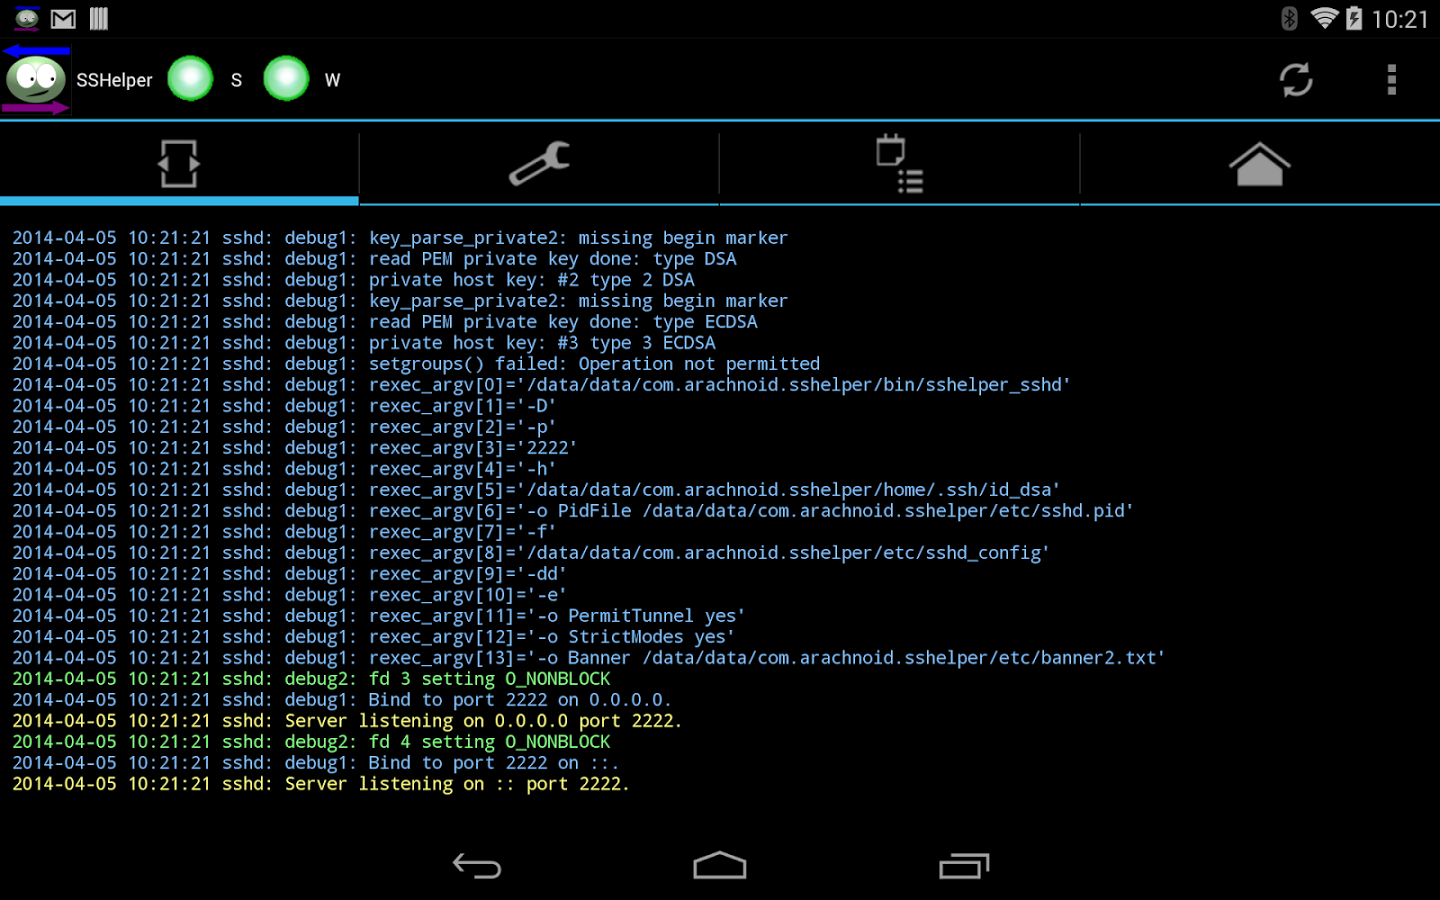
\includegraphics[width=0.6\textwidth]{imagenes/fig47.png}
    \caption{Modificación del archivo menu usando SSHelper}
  \end{center}
\end{figure}


Al modificar el archivo de alertas mientras la aplicación corría, esta mostró igualmente el menú de alertas sin problemas y el fichero se reescribió.